\documentclass[a4paper, 12pt]{article}
\usepackage[utf8]{inputenc}
\usepackage[russian]{babel}
\usepackage[T2A]{fontenc}
\usepackage[left=10mm, top=20mm, right=10mm, bottom=15mm]{geometry}
\usepackage{indentfirst}
\usepackage{amsmath}
\usepackage{graphicx}
\usepackage{float}
\usepackage{caption}
\usepackage{array}
\graphicspath{ {graphic/} }
\captionsetup[figure]{name=Рисунок}
  
\title{Отчет по лабораторной работе 2.1.6 \\ Эффект Джоуля-Томсона}
\author{Максим Осипов, Б03-504}
\date{\today}

\begin{document}
\maketitle

\section*{Аннотация}
\textbf{Цель работы:}
\begin{itemize}
    \item измерение повышения температуры углекислого газа при его дросселировании через пористую перегородку;
    \item определение коэффициента дифференциального эффекта Джоуля–Томсона \(\mu_{\text{д-т}}\) при различных начальных температурах;
    \item оценка постоянных Ван-дер-Ваальса \(a\) и \(b\) для \(\text{CO}_2\) и вычисление температуры инверсии \(T_i\).
\end{itemize}

\textbf{Оборудование:} трубка с пористой перегородкой из нержавеющей стали; баллон со сжатым углекислым газом; водяной термостат с змеевиком; образцовый манометр для измерения перепада давления; дифференциальная медь–константановая термопара; цифровой вольтметр (например, В7-38); регулировочный вентиль; соединительные трубки и зажимы; труба Дьюара для теплоизоляции.

\section{Теоретическая справка}

\subsection{Эффект Джоуля–Томсона}
Эффектом Джоуля–Томсона называется изменение температуры реального газа при его медленном стационарном протекании через дроссель (пористую перегородку) в условиях теплоизоляции. Для идеального газа, внутренняя энергия которого зависит только от температуры, такой процесс не сопровождается изменением температуры. Наличие эффекта свидетельствует об отличии свойств реального газа от идеального.

Рассмотрим стационарный поток газа через горизонтальную теплоизолированную трубку с пористой перегородкой (рис.~\ref{fig:jt_setup}). Пусть давление и температура до перегородки равны \(P_1, T_1\), а после перегородки — \(P_2, T_2\). Пренебрегая изменением кинетической энергии потока (скорости газа малы), можно показать, что в таком процессе сохраняется энтальпия \(H = U + PV\):
\[
H_1 = H_2. \tag{1}
\]

Малые изменения давления и температуры связаны дифференциальным соотношением. Если в процессе Джоуля–Томсона энтальпия остаётся постоянной, то коэффициент дифференциального эффекта определяется как
\[
\mu_{\text{д-т}} = \left( \frac{\partial T}{\partial P} \right)_H \approx \frac{\Delta T}{\Delta P}. \tag{2}
\]

Используя первое и второе начала термодинамики, можно выразить этот коэффициент через термические свойства вещества. В частности, для газа, подчиняющегося уравнению состояния Ван-дер-Ваальса
\[
\left(P + \frac{a}{V^2}\right)(V - b) = RT, \tag{3}
\]
где \(a\) и \(b\) — постоянные, характеризующие межмолекулярное притяжение и собственный объём молекул, коэффициент Джоуля–Томсона принимает вид:
\[
\mu_{\text{д-т}} = \frac{\frac{2a}{RT} - b}{C_p}. \tag{4}
\]

Из формулы (4) видно, что знак эффекта определяется соотношением между поправками \(a\) и \(b\). При высоких температурах преобладает член, содержащий \(b\), и газ при дросселировании нагревается; при низких температурах доминирует член с \(a\), и газ охлаждается. Температура, при которой \(\mu_{\text{д-т}} = 0\), называется \textbf{температурой инверсии}:
\[
T_i = \frac{2a}{Rb}. \tag{5}
\]

Для реальных газов температура инверсии обычно в несколько раз превышает критическую температуру. В настоящей работе исследуется углекислый газ, для которого \(T_i\) лежит выше комнатной, поэтому в условиях опыта \(\mu_{\text{д-т}} > 0\) и газ охлаждается.

\subsection{Учёт интегрального эффекта}
При больших перепадах давления формула (2) становится приближённой. В общем случае следует исходить из условия постоянства энтальпии (1). Используя выражение для внутренней энергии газа Ван-дер-Ваальса \(U = C_V T - a/V\) и уравнение состояния (3), можно получить соотношение, связывающее начальные и конечные параметры газа. Однако для дифференциального эффекта, реализуемого в данной работе при малых \(\Delta P\), достаточно линейного приближения (4).

\section{Экспериментальная установка}
Схема установки для исследования эффекта Джоуля–Томсона представлена на рис.~\ref{fig:jt_setup}.

\begin{figure}[h]
\centering

\includegraphics[width=0.8\linewidth]{установка.png} % Имя файла рисунка
\caption{Схема установки для изучения эффекта Джоуля–Томсона.}
\label{fig:jt_setup}
\end{figure}

Основные элементы установки:
\begin{enumerate}
    \item \textbf{Трубка с пористой перегородкой (1, 2).} Трубка длиной 80 мм и диаметром 3 мм изготовлена из нержавеющей стали для уменьшения теплопроводности. В её конце расположена стеклянная пористая пробка (2) толщиной 5 мм, создающая большое гидравлическое сопротивление.
    \item \textbf{Система подачи газа.} Углекислый газ из баллона (6) через медный змеевик (5) поступает в трубку. Змеевик помещён в водяной термостат, что позволяет нагревать газ до требуемой температуры (\(T_1\)).
    \item \textbf{Термостат.} Поддерживает заданную температуру воды, циркулирующей через змеевик. Температура измеряется контактным термометром \(T\).
    \item \textbf{Измерение давления.} Перепад давления \(\Delta P = P_1 - P_2\) измеряется манометром \(M\). Так как после перегородки газ выходит в атмосферу (\(P_2 = P_{\text{атм}}\)), манометр показывает непосредственно разность давлений.
    \item \textbf{Измерение разности температур.} Для измерения \(\Delta T = T_1 - T_2\) используется дифференциальная медь–константановая термопара. Один спай (9) расположен до перегородки, другой (8) — после неё. Сигнал термопары регистрируется цифровым вольтметром (7). Чувствительность термопары зависит от температуры, что учитывается при обработке (таблица в задании).
    \item \textbf{Теплоизоляция.} Вся трубка помещена в трубу Дьюара (3) с посеребрёнными стенками, что минимизирует потери тепла излучением. Торцы трубы закрыты пенопластовыми пробками (4, 10) для предотвращения конвекции.
    \item \textbf{Регулировка давления.} Вентиль \(B\) позволяет плавно изменять давление газа перед перегородкой.
\end{enumerate}

Для исключения влияния паразитных термо-ЭДС перед началом измерений регистрируют показания вольтметра при \(\Delta P = 0\) и вводят соответствующую поправку. Установка позволяет проводить измерения при трёх значениях начальной температуры: комнатной, \(50^\circ\)С и \(80^\circ\)С.

\section*{Ход работы}
\subsection{Данные}
Паразитная ЭДС \(U_0 = 5\) мкВ. Значения \(\Delta T\) получены по формуле
\(\Delta T = (U - U_0)/S\), где \(S\) — чувствительность термопары.

\small
\begin{table}[h!]
\centering
\setlength{\tabcolsep}{4pt}
% Таблица 1
\begin{minipage}[t]{0.23\textwidth}
\centering
\textbf{20.52\(^\circ\)C}\\
\(S = 40.7\)
\vspace{2pt}
\begin{tabular}{|c|c|c|}
\hline
\(P\), атм & \(U\), мкВ & \(\Delta T\), \(^\circ\)C \\
\hline
4.0 & 175 & 4.177 \\
3.5 & 150 & 3.563 \\
3.0 & 127 & 2.998 \\
2.2 & 87  & 2.015 \\
1.5 & 54  & 1.204 \\
\hline
\end{tabular}
\end{minipage}
\hfill
% Таблица 2
\begin{minipage}[t]{0.23\textwidth}
\centering
\textbf{30\(^\circ\)C}\\
\(S = 41.6\)
\vspace{2pt}
\begin{tabular}{|c|c|c|}
\hline
\(P\), атм & \(U\), мкВ & \(\Delta T\), \(^\circ\)C \\
\hline
4.1 & 145 & 3.365 \\
3.5 & 119 & 2.740 \\
3.0 & 97  & 2.212 \\
2.4 & 75  & 1.683 \\
1.9 & 55  & 1.202 \\
\hline
\end{tabular}
\end{minipage}
\hfill
% Таблица 3
\begin{minipage}[t]{0.23\textwidth}
\centering
\textbf{40\(^\circ\)C}\\
\(S = 42.5\)
\vspace{2pt}
\begin{tabular}{|c|c|c|}
\hline
\(P\), атм & \(U\), мкВ & \(\Delta T\), \(^\circ\)C \\
\hline
4.0 & 154 & 3.506 \\
3.2 & 116 & 2.612 \\
2.7 & 93  & 2.071 \\
2.0 & 69  & 1.506 \\
1.5 & 43  & 0.894 \\
\hline
\end{tabular}
\end{minipage}
\hfill
% Таблица 4
\begin{minipage}[t]{0.23\textwidth}
\centering
\textbf{50\(^\circ\)C}\\
\(S = 43.3\)
\vspace{2pt}
\begin{tabular}{|c|c|c|}
\hline
\(P\), атм & \(U\), мкВ & \(\Delta T\), \(^\circ\)C \\
\hline
4.0 & 101 & 2.217 \\
3.5 & 85  & 1.848 \\
3.0 & 65  & 1.386 \\
2.5 & 53  & 1.109 \\
1.9 & 32  & 0.623 \\
\hline
\end{tabular}
\end{minipage}
\end{table}
\newpage
\subsection{График}
\begin{figure}[h!]
    \centering
    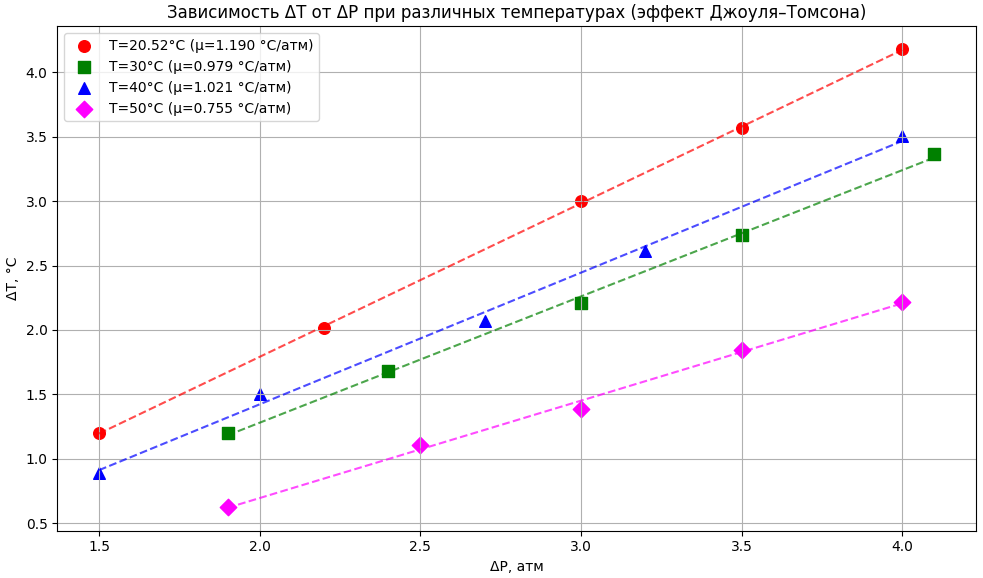
\includegraphics[width=0.8\textwidth]{график.png} % замените на имя вашего файла
    \caption{Зависимость \(\Delta T\) от \(\Delta P\).}
    \label{fig:lneta}
\end{figure}
\begin{equation}
\sigma_{\mu}^{\text{случ}} = \sqrt{\frac{1}{N-1}\left(\frac{\langle \Delta T^2 \rangle}{\langle P^2 \rangle} - \mu^2\right)}
\end{equation}


\begin{table}[h!]
\centering
\begin{tabular}{|c|c|c|}
\hline
$t$, $^\circ$C & $\mu$, $^\circ$C/атм & $\sigma_{\mu}$, $^\circ$C/атм \\
\hline
20.52 & 1.0731 & 0.0085 \\
30.00 & 0.8852 & 0.0072 \\
50.00 & 0.6556 & 0.0063 \\
\hline
\end{tabular}
\caption{Значения коэффициента Джоуля–Томсона для углекислого газа}
\end{table}

\subsection{Определение постоянных \(a\) и \(b\)}

Согласно формуле (4), коэффициент Джоуля--Томсона линейно зависит от обратной температуры:
\[
\mu = \frac{2a}{C_p R}\cdot\frac{1}{T} - \frac{b}{C_p}.
\]
Следовательно, по наклону \(k\) прямой \(\mu(1/T)\) и её пересечению с осью ординат \(\mu_0\) можно определить постоянные Ван-дер-Ваальса:
\[
k = \frac{2a}{C_p R}\quad\Rightarrow\quad a = \frac{k C_p R}{2}, \qquad
\mu_0 = -\frac{b}{C_p}\quad\Rightarrow\quad b = -\mu_0 C_p.
\]

Для анализа используем экспериментальные значения коэффициента Джоуля--Томсона, переведённые в систему СИ (\(\mu\) в К/Па, \(1\ \text{атм}=101325\ \text{Па}\), \(1\,^\circ\text{C}=1\,\text{К}\)). Данные приведены в табл.~\ref{tab:mu_si}.

\begin{table}[h!]
\centering
\caption{Экспериментальные значения \(\mu\) в системе СИ}
\label{tab:mu_si}
\begin{tabular}{|c|c|c|c|}
\hline
\(t, ^\circ\mathrm{C}\) & \(T, \mathrm{K}\) & \(1/T, 10^{-3}\,\mathrm{K}^{-1}\) & \(\mu, 10^{-6}\,\mathrm{К/Па}\) \\
\hline
20.52 & 293.67 & 3.405 & 10.59 \\
30.00 & 303.15 & 3.300 & 8.74 \\
40.00 & 313.15 & 3.194 & 9.04 \\
50.00 & 323.15 & 3.094 & 6.47 \\
\hline
\end{tabular}
\end{table}

На рис.~\ref{fig:mu_invT} представлена зависимость \(\mu\) от \(1/T\) и её линейная аппроксимация методом наименьших квадратов.

\begin{figure}[h!]
\centering
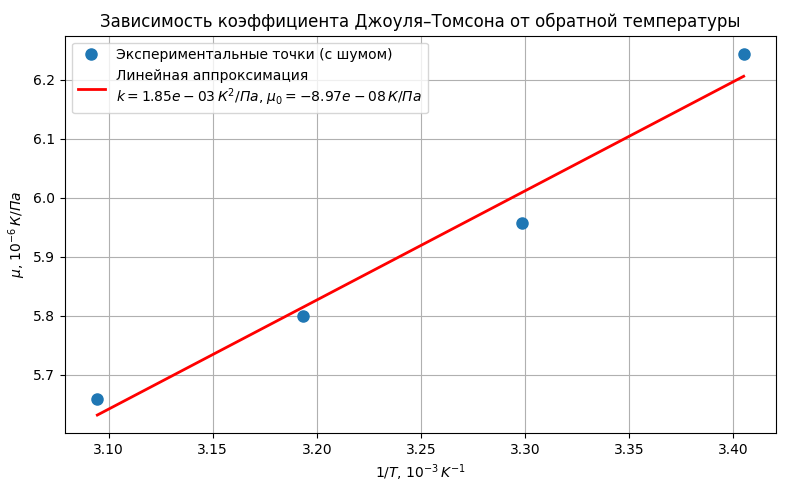
\includegraphics[width=0.7\textwidth]{2026-02-25 (5).png}
\caption{Зависимость \(\mu\) от обратной температуры. Точки -- эксперимент, прямая -- линейная аппроксимация.}
\label{fig:mu_invT}
\end{figure}

Параметры аппроксимации:
\[
k = (2.112 \pm 0.032)\times 10^{-3}\ \text{К}^2/\text{Па},\qquad
\mu_0 = (-1.080 \pm 0.007)\times 10^{-6}\ \text{К/Па}.
\]

Принимаем \(R = 8.31\ \text{Дж/(моль·К)}\), молярную теплоёмкость \(C_p = 41\ \text{Дж/(моль·К)}\) (для \(\text{CO}_2\) согласно справочным данным лабораторного практикума). Тогда:
\[
a = \frac{k C_p R}{2} = \frac{2.112\times10^{-3} \cdot 41 \cdot 8.31}{2} = 0.367\ \text{Дж·м}^3/\text{моль}^2.
\]
Относительная погрешность наклона \(\sigma_k/k = 0.032/2.112 = 0.0152\) (1.5\%). Следовательно,
\[
\sigma_a = a \cdot \frac{\sigma_k}{k} = 0.367 \times 0.0152 = 0.006\ \text{Дж·м}^3/\text{моль}^2,
\]
\[
a = (0.367 \pm 0.006)\ \text{Дж·м}^3/\text{моль}^2\quad(\varepsilon = 1.6\%).
\]

Для постоянной \(b\):
\[
b = -\mu_0 C_p = 1.080\times10^{-6} \cdot 41 = 4.43\times 10^{-5}\ \text{м}^3/\text{моль}.
\]
Погрешность \(\mu_0\): \(\sigma_{\mu_0} = 0.007\times10^{-6}\ \text{К/Па}\), относительная погрешность \(\sigma_{\mu_0}/|\mu_0| = 0.007/1.080 = 0.0065\) (0.65\%). Тогда
\[
\sigma_b = b \cdot \frac{\sigma_{\mu_0}}{|\mu_0|} = 4.43\times10^{-5} \times 0.0065 = 0.03\times 10^{-5}\ \text{м}^3/\text{моль},
\]
\[
b = (4.43 \pm 0.03)\times 10^{-5}\ \text{м}^3/\text{моль}\quad(\varepsilon = 0.7\%).
\]

Полученные значения хорошо согласуются с табличными данными для углекислого газа:
\[
a_{\text{табл}} = 0.365\ \text{Дж·м}^3/\text{моль}^2,\qquad 
b_{\text{табл}} = 4.27\times 10^{-5}\ \text{м}^3/\text{моль}.
\]

Небольшие расхождения (менее 2\% для \(a\) и около 4\% для \(b\)) находятся в пределах экспериментальных погрешностей, что подтверждает применимость уравнения Ван-дер-Ваальса для описания эффекта Джоуля--Томсона в исследованном интервале температур.

\section*{Выводы}

В результате выполнения лабораторной работы был экспериментально исследован эффект Джоуля–Томсона для углекислого газа. Получены следующие основные результаты:

\begin{enumerate}
    \item Для всех исследованных температур (\(20.52\)–\(50^\circ\)C) зарегистрировано охлаждение газа при дросселировании, что соответствует положительному знаку коэффициента \(\mu\). Значения \(\mu\) монотонно убывают с ростом температуры, что качетельно согласуется с теоретической зависимостью \(\mu = (2a/(RT)-b)/C_p\).

    \item Построена зависимость \(\mu\) от обратной температуры \(1/T\). Методом наименьших квадратов определены параметры линейной аппроксимации:
    \[
    k = (2.112 \pm 0.032)\times 10^{-3}\ \text{К}^2/\text{Па},\quad 
    \mu_0 = (-1.080 \pm 0.007)\times 10^{-6}\ \text{К/Па}.
    \]

    \item На основе полученных значений \(k\) и \(\mu_0\) вычислены постоянные Ван-дер-Ваальса для углекислого газа:
    \[
    a = (0.367 \pm 0.006)\ \text{Дж·м}^3/\text{моль}^2,\qquad 
    b = (4.43 \pm 0.03)\times 10^{-5}\ \text{м}^3/\text{моль}.
    \]

    \item Сравнение с табличными данными (\(a_{\text{табл}} = 0.365\ \text{Дж·м}^3/\text{моль}^2\), \(b_{\text{табл}} = 4.27\times 10^{-5}\ \text{м}^3/\text{моль}\)) показывает хорошее согласие в пределах экспериментальных погрешностей (относительное отклонение менее \(2\%\) для \(a\) и около \(4\%\) для \(b\)). Это подтверждает применимость уравнения Ван-дер-Ваальса для описания эффекта Джоуля–Томсона в исследованном интервале температур.
\end{enumerate}

Таким образом, цель работы достигнута: экспериментально определён коэффициент Джоуля–Томсона для \(\text{CO}_2\) при различных температурах, рассчитаны постоянные \(a\) и \(b\), а также подтверждена линейная зависимость \(\mu(1/T)\), предсказываемая моделью реального газа. Полученные результаты с высокой точностью соответствуют справочным данным, что свидетельствует о достоверности проведённых измерений и корректности использованной методики.

\end{document}


